

\documentclass[11pt, oneside]{report}  %can try book instead    % use "amsart" instead of "article" for AMSLaTeX format
\usepackage[margin = 0.7in, bmargin = 1.1in, tmargin = 0.9in]{geometry}                     % See geometry.pdf to learn the layout options. There are lots.
\geometry{a4paper}                          % ... or a4paper or a5paper or ... 
%\geometry{landscape}                       % Activate for rotated page geometry
\usepackage[parfill]{parskip}           % Activate to begin paragraphs with an empty line rather than an indent
\usepackage{graphicx}               % Use pdf, png, jpg, or eps§ with pdflatex; use eps in DVI mode
                                % TeX will automatically convert eps --> pdf in pdflatex        
\usepackage{amssymb}
\usepackage{amsmath}
\usepackage{amsmath,mathtools}
\usepackage{array}
\usepackage{tabu}
\usepackage{bm}
\usepackage{wrapfig}
\usepackage{multirow}
\usepackage{physics}
\usepackage{hyperref}
\usepackage{listings}
\usepackage[utf8]{inputenc}
\usepackage[T1]{fontenc}
\usepackage{lmodern}
%\usepackage{graphicx} %already declared above
\usepackage{caption}
\usepackage{float}
\usepackage{floatrow}
\usepackage{subfig}
\usepackage{multicol}
\usepackage{xcolor}
\usepackage{pagecolor}
\usepackage{lipsum}  
\usepackage{mdframed}
\usepackage{verbatim}
\usepackage{slashed}
%\usepackage[compat=1.1.0]{tikz-feynman}
%\usepackage{animate}


\newcommand{\G}{\mathcal{G}}
\newcommand{\D}{\mathcal{D}}
\newcommand{\E}{\mathcal{E}}
\renewcommand{\S}{\mathcal{S}}
\newcommand{\M}{\mathcal{M}}
\newcommand{\K}{\mathcal{K}}
\renewcommand{\L}{\mathcal{L}}
\newcommand{\R}{\mathcal{R}}
\renewcommand{\P}{\mathcal{P}}
\newcommand{\vp}{\varphi}
\newcommand{\T}{\mathcal{T}}
\newcommand{\A}{\mathcal{A}}
\newcommand{\bs}{\boldsymbol}
\newcommand{\rspace}{\mathbb{R}}
\newcommand{\dd}{\mathrm{d}}


\definecolor{purple}{RGB}{38,0,75}
\pagecolor{white}
\color{black}

%SetFonts

%SetFonts
\usepackage{subfiles} % Best loaded last in the preamble

\numberwithin{equation}{section}
\pagenumbering{gobble}
\title{Third Term Report}
\author{Robin Croft}
%\date{}    
\begin{document}







%\newpage
%\pagenumbering{arabic}
\tableofcontents
\newpage




%\newpage
%\pagenumbering{arabic}




\section{Mathematical Modelling of Boson Stars}
\subsection{Action}
The Boson Stars considered are a complex Klein Gordon Scalar field, $\varphi$, minimally coupled to gravity. The action is the Einstein Hilbert vacuum action plus the matter action for curved space.
\begin{gather} S = \int_\mathcal{M}\left[\mathcal{L}_{EH} + \mathcal{L}_M\right] \sqrt{-g}\,\dd x^4 \\
 \L_{EH} = \frac{1}{16\pi G}R \\
 \L_{M} =-\frac{1}{2}g^{\mu\nu}\nabla_\mu \varphi^* \nabla_\nu \varphi - \frac{1}{2}V(|\varphi|^2)  \end{gather}
Here $V$ is the Klein-Gordon potential and it's effect on boson stars is discussed in [].
\begin{align}
V &= \frac{m^2 c^2}{\hbar^2 }|\vp|^2 \rightarrow m^2 |\vp|^2\\
V &= \frac{m^2 c^2}{\hbar^2 }|\vp|^2 + \frac{1}{2}\Lambda|\vp|^4 \rightarrow m^2|\vp|^2 + \frac{1}{2}\Lambda|\vp|^4\\
V &= \frac{m^2 c^2}{\hbar^2 }|\vp|^2\left(1-\frac{|\vp|^2}{2\sigma^2}\right)^2 \rightarrow {m^2 }|\vp|^2\left(1-\frac{|\vp|^2}{2\sigma^2}\right)^2
\end{align}
Considering only the $m^2$ term, which corresponds to the squared mass of the particle in the quantum theory, we get a massive wave equation linear in $\varphi$, leading to so called mini Boson stars. Having $\Lambda\neq0$ gives self-interacting stars which have a nonlinear wave equation corresponding to particle creation and annihilation at the quantum level. Finally, equation 3.6 describes the solitonic potential, giving rise to boson stars with compactnesses comparable to neutron stars. 

Varying the action with respect to the metric and scalar field return the Einstein Field equations and the Klein Gordon equation of curved space respectively.
\begin{equation} R_{\mu\nu} - \frac{1}{2}R g_{\mu\nu} =  \frac{8\pi G}{c^4} T_{\mu\nu}  \end{equation}
\begin{equation}  g^{\mu\nu}\nabla_\mu\nabla_\nu \vp = \frac{\partial V}{\partial |\vp|^2}\vp \end{equation}
Collectively these are known as the Einstein-Klein-Gordon (EKG) equations. The definition and boson-specific stress energy tensors are as follows.
\begin{align}  
T_{\mu\nu} :&= -2\frac{\delta \mathcal{L}_{M}}{\delta g^{\mu\nu}}+g_{\mu\nu}\mathcal{L}_M \\
T_{\mu\nu} &= \frac{1}{2}\nabla_{\mu}\varphi^*\nabla_{\nu}\varphi+\frac{1}{2}\nabla_{\nu}\varphi^*\nabla_{\mu}\varphi-\frac{1}{2}g_{\mu\nu}\left[g^{\alpha\beta}\nabla_\alpha\varphi^*\nabla_\beta\varphi + V\right] 
\end{align}
Studying neutron stars requires the fermionic, or ordinary fluid, stress tensor; this is given below.
\begin{equation} T^{\mu\nu}_F = \left[\rho c^2+ {P} \right]\frac{u^\mu u^\nu}{c^2} + P g^{\mu\nu} + 2u^{(\mu}q^{\nu)}+\pi^{\mu\nu}\end{equation} 
The vanishing of the divergence, $\nabla_\nu T^{\mu\nu}=0 $, returns the highly nonlinear relativistic Navier-Stokes equations of curved space. The viscosity term $\pi^{\mu\nu}$ and heat flux $q^\mu$ are often omitted for simplicity. The remaining variables $\rho$, $P$ and $u^\mu$ are the fluid density [and enthalpy?], pressure and worldline tangent. Note here the use of sophisticated shock capturing schemes are required, unlike the linear Klein-Gordon equation.


\subsection{Solitons}
A soliton is a wave that exhibits particle-like behaviour. More precisely, in classical field theory, a soliton is a field or set of fields in a localised configuration that can travel at constant speed but not disperse. Some examples of solitons in General Relativity are fluid stars, black holes, wormholes and exotic stars [refernece]. [check are they solitons if they cannot pass though each other (e.g. black holes ...)]. For our purposes, we look for solitons in the Einstein-Klein Gordon (EKG) system which are localised scalar field configurations with accompanying metric. In the case of the real scalar field it was shown by [] that there are no long lived stars; however promoting the field to a complex scalar we can find a spherically symmetric stationary soliton with the following scalar field.
$$ x^\mu \in \{t,r,\theta,\phi \}$$
\begin{equation} \varphi = \Phi(r)e^{i\omega t} \end{equation}
Traditionally, the polar areal gauge has been used [] for the metric's ansatz.
\begin{equation}g_{\mu\nu}\dd x^\mu \dd x^\nu =- a^2(r)\dd t^2 + b^2(r) \dd r^2 + r^2 \left[ \dd \theta^2 + \sin^2\theta \dd \phi^2\right]\end{equation}
The boundary condition $b^2(0)=1$ is demanded to avoid a conical singularity at the origin. However an isotropic gauge is more useful for simulations due to easier conversion to cartesian space-coordinates. The polar areal solution must then be transformed into an isotropic solution. Alternatively, the approach taken in this report, is to start with an isotropic ansatz
\begin{equation} g_{\mu\nu}\dd x^\mu \dd x^\nu =- \Omega^2(r)\dd t^2 + \Psi^2(r)\dd \bm{x}^2\end{equation}
where $\dd \bm{x}^2$ denotes the euclidean 3D line element; this changes between spherical polar or cartesian coordinates trivially. This ends up being slightly harder to integrate numerically, but no conversion to isotropic coordinates is needed afterwards.

To get a set of ODE's to solve for the functions $\{\Omega(r), \Psi(r),\Phi(r)\}$ we must turn to the Einstein Equation and Klein Gordon Equation. The Einstein Equations for $\{\mu,\nu\}=\{0,0\},\{1,1\},\{2,2\}$ are the only components that give unique non-zero equations; they are given below.
\begin{gather}
\frac{\Omega ^2 \left[r \Psi '^2-2 \Psi  \left[r \Psi ''+2 \Psi '\right]\right]}{r \Psi ^4} = 4\pi G \left[\Omega ^2 \left[\frac{P'^2}{\Psi ^2}+V\right]+\omega ^2 P^2\right]\\
\frac{2 \Psi  \Psi ' \left[r \Omega '+\Omega \right]+r \Omega  \Psi '^2+2 \Psi ^2 \Omega
   '}{r \Psi ^2 \Omega } = 4\pi G \left[P'^2-\Psi ^2 V+\frac{\omega ^2 P^2 \Psi ^2}{\Omega
   ^2}\right]\\
   r \left[-\frac{r \Psi '^2}{\Psi ^2}+\frac{r \Psi ''+\Psi '}{\Psi }+\frac{r \Omega ''+\Omega
   '}{\Omega }\right] = -4\pi G r^2 \Psi ^2 \left[\frac{P'^2}{\Psi ^2}+V-\frac{\omega ^2 P^2}{\Omega
   ^2}\right]
   \end{gather}
  The Einstein tensor $G_{\mu\nu} = R_{\mu\nu}-\frac{1}{2}R g_{\mu\nu}$ (left above) and the stress tensor (right above) were obtained with a self written Mathematica notebook. The Klein Gordon equation (3.6) becomes
  \begin{gather*} \frac{1}{\sqrt{-g}}\partial_\mu \left[ \sqrt{-g}g^{\mu\nu}\partial_\nu \Phi(r)e^{i\omega t}\right] = \frac{\partial V}{\partial |\vp|^2} \Phi(r)e^{i\omega t} \\
  \Phi'' = \Phi\Psi^2\left[V'-\frac{\omega^2}{\Omega^2}\right] - \Phi'\left[\frac{\Omega'}{\Omega} +\frac{\Psi'}{\Psi}+\frac{2}{r} \right]\end{gather*}
Simplifying the Einstein Equations and combinig with the Klein Gordon equation we get 3 ODE's to solve.
\begin{gather}\Omega '=\frac{\Omega}{r\Psi'+\Psi}\left[2 \pi  G r \Psi \left[\Phi'^2 -\Psi^2 
   V+\frac{\omega ^2 \Phi^2 \Psi^2}{\Omega^2} \right]  -\Psi '-\frac{r \Psi '^2}{2 \Psi} \right]
\\{ \Psi'' = \frac{\Psi'^2}{2\Psi} - \frac{2\Psi'}{r}-2\pi G \left[V \Psi^3 + \Phi'^2\Psi+ \frac{ \omega^2\Phi^2\Psi^3}{\Omega^2}\right] }
\\ \Phi'' = \Phi\Psi^2\left[V'-\frac{\omega^2}{\Omega^2}\right] - \Phi'\left[\frac{\Omega'}{\Omega} +\frac{\Psi'}{\Psi}+\frac{2}{r} \right]\end{gather}
This is turned into a set of five first order ODE's to numerically integrate. Note that if we had used the polar areal ansatz () the equation for $\Phi$ would also be first order; reducing the EKG system to four first order ODE's.

\subsection{3+1 Klein Gordon System}
Now let's project the Klein Gordon equation in a 3+1 split to get an evolution equation. The first step is to turn the second order (in time) differential equation into two first order ones
\begin{equation} \L_m \{\vp,\Pi \} = ...\end{equation}
where $\Pi$ is the foliation dependant definition of conjugate momentum to the complex scalar field.
\begin{equation} \Pi:= -\L_n \vp\end{equation}
Now decompose the Klein Gordon Equation.
\begin{equation} \nabla^\mu \nabla_\mu \vp = V' \vp = \frac{1}{\sqrt{-g}} \partial_\mu \left[ \sqrt{-g}\left[\gamma^{\mu\nu}-n^\mu n^\nu\right]\partial_\nu \vp\right] = \frac{1}{\sqrt{-g}} \partial_\mu \left[ \sqrt{-g}\left[\D^\mu\vp-n^\mu \L_n\vp\right]\right] \end{equation}
The term with $\D^\mu$ simplifies like
\begin{equation}\frac{1}{\sqrt{-g}} \partial_\mu \left[ \sqrt{-g}\D^\mu\vp\right] =  \frac{1}{\alpha\sqrt{\gamma}} \partial_\mu \left[\alpha\sqrt{\gamma}\D^\mu\vp\right]  = \D_\mu \D^\mu \vp + \D^\mu \vp \,\partial_\mu \ln \alpha\end{equation}
and the remainder becomes
\begin{equation}-\frac{1}{\sqrt{-g}} \partial_\mu \left[ \sqrt{-g}n^\mu \L_n\vp\right] = -\left[\nabla \cdot n + n\cdot \partial\right]\L_n\vp = -\K\Pi + \L_n \Pi\end{equation}
then the full Klein Gordon system is constructed.
\begin{align}
 \L_m \Pi &= - \D^\mu\vp\,\partial_\mu \alpha+\alpha\left[\K\Pi - \D_\mu \D^\mu \vp  + V'\vp\right] \\
 \L_m \vp &= - \alpha\Pi\end{align}
The final matter term we must decompose is the Klein-Gordon stress tensor with equations (). \begin{align} E &=n^\mu n^\nu T_{\mu\nu} = \frac{1}{2}|\Pi|^2 + \frac{1}{2}\gamma^{ij}\D_i \varphi^* \D_j \varphi +\frac{1}{2}V(|\varphi|^2)
\\ S_i &= -\perp^\mu_i n^\nu T_{\mu\nu} =  \frac{1}{2}\left[\Pi^* \D_i \vp  +  \Pi\D_i \vp^* \right]
\\ S_{ij} &= \perp^\mu_i \perp^\nu_j T_{\mu\nu} = \D_{(i}\vp\D_{j)}\vp^* - \frac{1}{2}\left[ \gamma^{ij}\D_i\vp\D_j\vp^* - |\Pi|^2 + V(|\vp|^2)\right]\end{align}

\subsection{Klein Gordon's Noether Charge}
For the complex scalar field, we have the U(1) symmetry
\begin{equation}\vp \rightarrow \vp e^{i\epsilon} \approx \vp + i\epsilon \vp , \quad\vp^* \rightarrow \vp^* e^{-i\epsilon}  \approx \vp^* - i\epsilon \vp*.\end{equation}
This leaves the Lagrangian unchanged and therefore the total action. The associated conserved current $j$ and current density $\mathcal{J}$ are then
\begin{align*} j^\mu &= \frac{\delta \L}{\delta \nabla_\mu\vp}\delta \vp + \frac{\delta \L}{\delta \nabla_\mu \vp^*}\delta \vp*, \quad \nabla_\mu j^\mu =0,\\
 j^\mu &=  ig^{\mu\nu}\left[\vp\nabla_\nu\vp^* - \vp^*\nabla_\nu\vp\right], \quad \mathcal{J}^\mu = \sqrt{-g}j^\mu.\end{align*}
The total integral over a manifold $\M$ gives a conserved charge $\mathcal{Q}$ associated with the conserved current $J^\mu$, assuming $\mathcal{J}^i\rightarrow0$ sufficiently fast towards the boundary $\partial \Sigma_t$ of $\Sigma$.
\begin{equation}\int_\M \left[\nabla \cdot j\right] \star 1 = 0 = \int_{\phi(\M)} \nabla_\mu j^\mu \sqrt{-g}\,\dd x^4 = \int_{\phi(\M)} \partial_\mu \left[\sqrt{-g} j^{\mu} \right] \dd x^4= \int_{\phi(\M)}\partial_\mu \mathcal{J}^\mu \dd x^4\end{equation}
\begin{equation} \int^{t_1}_{t_0}\left[\int_{\phi(\Sigma_t)} \partial_0 \mathcal{J}^0 \dd x^3 \right]\dd t = -\int^{t_1}_{t_0}\left[\int_{\phi(\Sigma_t)} \partial_i \mathcal{J}^i \dd x^3 \right]\dd t = 0\end{equation}
The term containing $\partial_i\mathcal{J}^i$ integrates to zero over $\Sigma_t$ due to the divergence theorem. The left hand term can be simplified by permuting the time derivative using
\begin{equation} \partial_0 \int_{\phi(\Sigma_t)}\mathcal{J}^0 \dd x^3 = \int_{\phi(\Sigma_t)}\partial_0 \mathcal{J}^0 \dd x^3 + \lim_{\Delta x^0\rightarrow0}\left[ \frac{1}{\Delta x^0}\int_{\phi(\Delta \Sigma_t)}\left[ \mathcal{J}^0 +\Delta x^0 \partial_0 \mathcal{J}^0\right] \dd x^3 \right]\end{equation}
where the last term vanishes as $\mathcal{J}$ vanishes near $\partial\Sigma$, and we get a formula for the conserved charge.
\begin{equation} \partial_0 \int \mathcal{Q}=0, \quad \mathcal{Q} = \int_{\phi(\Sigma_t)}\mathcal{J}^0 \dd x^3 \end{equation}
Finally we get an expression for the total Noether charge $\mathcal{N} = \mathcal{Q}[\vp]$
\begin{equation}\mathcal{N} =i \int_{\Sigma_t} \sqrt{-g}\left[ \vp \nabla^0 \vp^* - \vp^*\nabla^0 \vp\right] \dd x^3\end{equation}
and using $\sqrt{-g} = \alpha \sqrt{\gamma}$, $n_\mu \nabla^\mu = -\alpha \nabla^0$ we get the following neat formula.
\begin{equation} \mathcal{N} = i\int_{\Sigma_t}\left[ \vp \Pi^*-\vp^*\Pi\right] \sqrt{\gamma}\,\dd x^3\end{equation}

MAYBE POINT THIS SECTION AT THE CONTINUITY PAPER, OR JSUT SAY WE GENERALISE IT IN THERE?

\subsection{Boosted Boson Stars and Black Holes}
Let us now consider a moving star, this corresponds to making a stationary soliton and boosting it. There is no unique way of doing this as any coordinate transformation that reduces to a Minkowski spacetime boost at large radius will do the job. All the degrees of freedom we have can be absorbed into a coordinate gauge choice, so it makes sense to choose the trivial boost, with rapidity $\chi$, from Special Relativity.
\begin{equation}\chi=\mathrm{arctanh} \frac{v}{c}\end{equation}
\begin{equation}\Lambda_\nu^\mu =  \exp\begin{pmatrix} 0 & -\chi & 0& 0 \\ -\chi & 0 & 0 & 0\\ 0 & 0&1&0 \\ 0&0&0&1\end{pmatrix} = \begin{pmatrix} \cosh(\chi) & -\sinh(\chi) & 0& 0 \\ -\sinh(\chi) & \cosh(\chi) & 0 & 0\\ 0 & 0&1&0 \\ 0&0&0&1\end{pmatrix} \end{equation}
\begin{equation}\tilde{x}^\mu = \Lambda_{\nu}^{\mu}x^{\nu}\quad \& \quad \tilde{g}_{\mu\nu} = [\Lambda^{-1}]^\alpha_\mu[\Lambda^{-1}]^\beta_\nu g_{\alpha\beta}(\tilde{x}) \end{equation}
Declaring the rest and boosted frame to have coordinates $x^\mu$ and $\tilde{x}^\mu$ we choose the boosted soliton's initial Cauchy surface to be the level set of $\tilde{t}=0$. The coordinates and metric transform as follows.
\begin{align*} x^\mu &= \{ t,x,y,z\} = \{\tilde{t}\cosh(\chi) + \tilde{x} \sinh(\chi),\tilde{x}\cosh(\chi)+\tilde{t}\sinh(\chi),\tilde{y},\tilde{z}\} \\
 g_{\mu\nu} &= \mathrm{diag} \{ -\Omega^2, \Psi^2,  \Psi^2, \Psi^2\} \\
 \tilde{g}_{\mu\nu}&=\begin{pmatrix} -\Omega^2\cosh^2 (\chi) + \Psi^2 \sinh^2 (\chi) & \sinh(\chi)\cosh(\chi)\left[\Omega^2-\Psi^2\right] & 0& 0 \\  \sinh(\chi)\cosh(\chi)\left[\Omega^2-\Psi^2\right] & \Psi^2 \cosh^2 (\chi) - \Omega^2 \sinh^2 (\chi) & 0 & 0\\ 0 & 0&\Psi^2&0 \\ 0&0&0&\Psi^2\end{pmatrix}\end{align*}
Comparing this boosted metric to the $3+1$ decomposed metric () we can read off the shift vector $\tilde{\beta}_i$, the 3 metric $\tilde{\gamma}_{ij}$ and obtain the lapse and metric determinant.
\begin{equation} \tilde{\alpha}^2 = \frac{\Psi ^2 \Omega ^2}{\Psi ^2 \cosh ^2(\chi) -\Omega ^2 \sinh ^2(\chi) } \end{equation}
\begin{equation}\tilde{\gamma} = \det \tilde{\gamma}_{ij} = \Psi^4\left[ \Psi^2 \cosh^2 (\chi) - \Omega^2 \sinh^2(\chi)\right]\end{equation}
Finally, the conformal 3-metric with unit determinant is 
\begin{equation} \bar{\gamma}_{ij} = \tilde{\gamma}^{-\frac{1}{3}}\left(
\begin{array}{ccc}
 \Psi ^2 \cosh ^2(\chi) -\Omega ^2 \sinh ^2(\chi)  & 0 & 0 \\
 0 & \Psi ^2 & 0 \\
 0 & 0 & \Psi ^2 \\
\end{array}
\right).\end{equation}
Note normally $\tilde{\gamma}_{ij}$ is the conformal 3-metric, but to avoid confusion with the boosted frame it is denoted $\bar{\gamma}_{ij}$. Turning our attention to the matter fields now we only need to change the coordinate dependance, like $\vp(x)\rightarrow \vp(\tilde{x})$, and remembering $\tilde{t}=0$ defines our boosted frame, which implies $t = \tilde{x}\sinh(\chi)$, we get the following boosted complex scalar field.
\begin{equation}\vp = \Phi(\tilde{x}^2\cosh^2(\chi) +\tilde{y}^2 + \tilde{z}^2)e^{i\omega \tilde{x}\sinh(\chi)} \end{equation}
Note the field is modulated by an oscillatory phase now with wavenumber $k = \omega \tilde{x} \sinh(\chi)$; nodal planes in $\Re(\vp)$ appear perpendicular to velocity. The conjugate momentum $\tilde{\Pi}$ () in the boosted frame it becomes 
\begin{equation} \tilde{\Pi}(\tilde{x}^\mu) = -\L_{\tilde{n}} \vp(\tilde{x}^\mu)=-\frac{1}{\tilde{\alpha}}\tilde{m}\cdot \tilde{\partial}\vp = -\frac{1}{\tilde{\alpha}}\left[ \tilde{\partial}_0 - \tilde{\beta}^i\tilde{\partial}_{i}\right]\Phi(r)e^{i\omega t}.\end{equation}
Inconveniently we cannot simply evaluate $\tilde{\Pi}$ in the rest frame as this has a different spacetime foliation and the normal vector $n\neq \tilde{n}$ is genuinely changed; not just transforming components under coordinate transformation. Explicitly writing the contravariant components of the shift vector 
\begin{equation} \tilde{\beta}^i = \left(\frac{\sinh (\chi)  \cosh (\chi)  \left[\Omega ^2-\Psi ^2\right]}{\Psi ^2 \cosh
   ^2(\chi) -\Omega ^2 \sinh ^2(\chi) },0,0\right)\end{equation}
and the partial derivatives of $\vp$ in the boosted frame
\begin{equation} \tilde{\partial}_{0} = \cosh(\chi) \partial_t + \sinh(\chi) \partial_x,\quad 
\tilde{\partial}_{1} = \cosh(\chi) \partial_x + \sinh(\chi) \partial_t\end{equation} 
 \begin{equation}\partial_t\vp =\Phi\partial_te^{i\omega t} =i\omega \Phi e^{i\omega t},\quad
 \partial_x\vp =\frac{\partial r}{\partial x}\Phi'e^{i\omega t} = \frac{x}{r}\Phi'e^{i\omega t} \end{equation}
we get an expression for the boosted conjugate momentum; explicitly setting $\tilde{t}=0$ gives the momentum on the surface $\tilde{t}=0$ to be used as initial conditions in GRChombo. 
\begin{equation} \widetilde{\Pi} = -\frac{1}{\tilde{\alpha}}\left[  \left[ \sinh(\chi)-\tilde{\beta}^1 \cosh(\chi)\right]\frac{\tilde{x}\cosh(\chi)}{r}\Phi' + i\omega \left[ \cosh(\chi)-\tilde{\beta}^1\sinh(\chi)\right]\Phi\right]e^{i\omega \tilde{x}\sinh(\chi)}\end{equation}
Our final ingredient is the intrinsic curvature, defined in ().
\begin{equation} \widetilde{\K}_{\mu\nu} := -\frac{1}{2}\L_{\tilde{n}}\tilde{\gamma}_{\mu\nu} =-\frac{1}{2\tilde{\alpha}}\L_{\tilde{m}}\tilde{\gamma}_{\mu\nu} = -\frac{1}{2\tilde{\alpha}}\left[ \tilde m \cdot \tilde{\partial}\tilde{\gamma}_{ij} +  \tilde{\gamma}_{ik}\tilde{\partial}_j \tilde{m}^k +\tilde{\gamma}_{jk}\tilde{\partial}_i \tilde{m}^k\right]\end{equation}
A self written mathematica script gives the following expansion.
\begin{align}\alpha^{-1} \widetilde{\K}_{xx} &= \cosh^2(\chi)\sinh(\chi)\frac{x \left[v^2 \Omega^2 \Omega'+\Psi \Omega \Psi'-2 \Psi^2 \Omega'\right]}{r \Psi^2 \Omega}\\
 \alpha^{-1} \widetilde{\K}_{xy} &= \cosh(\chi)\sinh(\chi)\frac{ y \left[\Omega \Psi'- \Psi \Omega'\right]}{r \Psi \Omega }\\
 \alpha^{-1} \widetilde{\K}_{xz} &= \cosh(\chi)\sinh(\chi)\frac{ z \left[\Omega \Psi'- \Psi \Omega'\right]}{r \Psi \Omega }\\
 \alpha^{-1} \widetilde{\K}_{yy} &= -\sinh(\chi)\frac{ x \Psi'}{ r \Psi }\\
\widetilde{\K}_{zz}&=\widetilde{\K}_{yy} \end{align}
Clearly we can apply this to the Black Hole spacetime by an identical procedure, but ignoring $\vp$ and $\Pi$ and setting the isotropic solutions
\begin{equation} \Omega = \frac{1-\frac{M}{2r}}{1+\frac{M}{2r}}, \quad  \quad \Psi = \left[1+\frac{M}{2r}\right]^2.\end{equation}
 
 \subsection{Spherical Harmonics in Curved Space}
 Spherical harmonics are an orthonormal function basis for the surface of a sphere. They arise when looking for solutions to the 3D spherical polar laplacian
 \begin{equation} \nabla^2 \vp= \frac{1}{\sqrt{|g|}}\partial_{\mu}\left( \sqrt{|g|}g^{\mu\nu}\partial_\nu \vp\right), \quad \mu,\nu \in \{1,2,3\} .\end{equation}
 On the hypersurface $r=1$ we get the following metric
 \begin{equation} g_{\mu\nu} = \begin{pmatrix} 1 & 0 \\ 0 & \sin^2 \theta\end{pmatrix},\end{equation}
 and on this surface the spherical harmonics $Y_{lm}(\theta,\phi)$ satisfy the following condition.
 \begin{equation} \D_\mu \D^\mu Y_{lm}(\theta,\phi) = -l(l+1)Y_{lm}(\theta,\phi), \quad x^\mu \in \{\theta,\phi\}\end{equation} 
 This means we can take any spherically symmetric and static metric with $g_{\phi\phi} = \sin^2\theta g_{\theta\theta}$ and replace the angular part of the wave equation with $l(l+1)$. For a spherically symmetric spacetime this gives the Klein Gordon equation for scalar hair.
 \begin{equation} \nabla_\mu \nabla^\mu \vp = V' \vp, \quad \vp = T(t)R(r)Y_{lm}(\theta,\phi)\end{equation}
 \begin{equation}\vp^{-1}\nabla_\mu \nabla^\mu \vp = g^{tt}\frac{\ddot{T}}{T} +  \frac{1}{R\sqrt{|g|}}\partial_{r}\left( \sqrt{|g|}g^{rr}\partial_r R\right) -{l(l+1)}g^{\theta\theta} \end{equation}
 This is a second order ODE for the radial profile $R$ and is an eigenvalue problem for $\omega$ if we assume $T=e^{i\omega t}$. Assuming $T=e^{-kt}$ can be done on-top of the black hole metric () and requires the assumption of no back reaction of the scalar field on the metric; this gives an eigenvalue problem in $k$ instead. This leads to the following ODE for the radial profile. 
 \begin{equation} \frac{1}{R\sqrt{|g|}}\partial_{r}\left( \sqrt{|g|}\Psi^{-4}\partial_r R\right)  = k^2 \frac{\Omega^2}{\Psi^2} + \frac{l(l+1)}{r^2 \Psi^4} + V'\end{equation}
Simulations shown later involve boson stars of mass $M$ and black holes of mass $M\rightarrow 10M$; these simulations often produce scalar hair about these black holes that is orders of magnitude less massive than the boson stars. In this regime the above equation is assumed relevant.


MAYBE JUST USE THIS SECTION TO TALK ABOUT THE COLLISIONS THAT MAYBE SEEM TO FOLLOW THIS RULE ... SAY HOW EVEN THOUGHT ITS NOT REALLY SPHERICALLY SYMMETRIC MAYBE IT CAN BE APPROXIMATES BY THIS? AND WE CAN'T USE SUPERPOSISION OF SOLUTIONS REALLY 













\section{Numerical Simulations}
\subsection{Introduction to Numerical Methods}

talk about stuff like eular step, unstable then runge kutta and stnecil derivatives and then method of lines



\subsection{GRChombo}
GRChombo [] is a recently developed Numerical Relativity code built on top of Chombo [], a PDE solver with fully adaptive mesh refinement (AMR). The advantage of AMR is that regridding, and subsequently sub-volumes of high resolution, is calculated during runtime. This is especially useful for simulating fluids in GR as they can develop features requiring higher resolution in places a human may not expect making pre-specified mesh refinement hard to use. GRChombo uses the CCZ4 system with 1+log slicing and the Gamma driver shift condition, discussed in sections (). GRChombo also supports vectorisation and parallelisation with OpenMP and MPI making it suitable for use on supercomputer clusters. 

So far I have implemented initial data for a single or binary system of compact objects which can be either a Schwarzschild black hole or a boson star. The initial data uses isotropic coordinates and can be boosted along coordinate axes, but not yet general directions, giving the possibility of single boosted objects, accelerated head on collisions, grazing collisions and inspirals/quasi-orbits. It should be noted that my implementation was built on top of the pre-existing complex scalar field class (written by Miren). The remainder of this section will cover the numerical aspects of my work.

TALK MORE ABOUT GRCHOMBO AND MAYBE REF THE NEW PAPER


\subsection{Simulation Units}
MAKE THIS WORK WITH THE CONVENTIONS SECTION ASND THEN DESCRIBE WHAT IS NEW FOR ONLY THE SIMULATIONS

GRChombo defaults to geometric units, as described in section (1.2). The scalar field $\vp$ appears in the action as
\begin{equation} S = \int_{\M} \left[g^{\mu\nu}\partial_\mu \vp \partial_\nu \vp^* + ... \right]\dd x^4\end{equation}
and given $S$ and the metric are dimensionless, dimensional analysis tells us $\vp$ has units of inverse length in natural units, or units of energy. The Klein-Gordon mass $m$
\begin{equation} \Box \vp = m^2 \vp\end{equation}
can be absorbed into new dimensionless spatial coordinates $\tilde{x}^i = x^i m$ changing the KG equation to the scale invariant form.
\begin{equation} \Box \vp = \vp\end{equation}



\subsection{Initial Data}
Following on from the EKG ODE's () we now seek to solve them numerically to obtain initial data for a single static boson star. The system can be reduced to a set of five first order ODE's so we have 5 boundary conditions. Intuitively, for a physical star we would like to impose $\Phi(0) = \Phi_c$, $\Phi'(0)=0$, $\Phi(r\rightarrow\infty)\rightarrow0$, $\Omega'(0)=0$, $\Omega(r\rightarrow\infty)\rightarrow1$, $\Psi'(0)=0$ and $\Psi(r\rightarrow\infty)\rightarrow1$ to be regular at the origin and match the Schwarzschild vacuum solution at large radius; however this is 7 boundary conditions. One of these can be removed by asking for asymptotic flatness, $\sqrt{\Psi(\infty)}\left(1+\Omega(\infty)\right)=2$, rather than $\Omega(\infty)=\Psi(\infty)=1$, which is inspired by the isotropic black hole metric. One final point of importance is the frequency $\omega$ turns the Klein-Gordon ODE () into an eigenvalue problem, admitting only discrete values of $\omega$.

The first attempt to find the radial profile $\{\Phi(r),\Omega(r),\Psi(r)\}$ of the boson star was to use a relaxation method as it trivially incorporates the above two-point boundary conditions. The modification of promoting equation () to a second order ODE like \begin{equation}\Omega''(r) = f(g_{\mu\nu},\partial g_{\mu\nu},\Phi,\partial \Phi)\end{equation}
is one way we can get an extra degree of freedom to allow 6 boundary conditions; it also means all the EKG ODE's can be written in a parabolic (heat/diffusion equation like) form
\begin{equation} \frac{\partial H}{\partial t}  = \nabla^2 H + f(H,...) \end{equation}
by introducing an imaginary time $t$ and solved iteratively via evolving in $t$ to a final state where $\dot{H}=0$ thus solving the ODE; this is a relaxation method. In practice this method did not work well with the eigenvalue problem in $\omega$. Unlike with a shooting method, there was no obvious way of telling whether the guess $\omega$ was bigger or smaller than the correct value. Even if this problem were overcome, numerical solution with relaxation takes far longer than than a simple shooting method, even with Chebychev acceleration [], hence a shooting method was chosen over relaxation.

To find the initial data for a single Boson star, a private c++ script was written using RK4 to integrate the EKG system taking 5 initial conditions, and eigenvalue guess $\omega_0$. 
\begin{equation} \{\Phi(0),\Phi'(0),\Psi(0),\Psi'(0),\Omega(0);\omega \} = \{ \Phi_c,0,\Psi_c,0,\Omega_c;\omega_0\}\end{equation}
Unfortunately we do not know $\Omega_c$ and $\Psi_c$ apriori, but it turns out that guessing any values, such as $\Omega_c=0.5$ and $\Psi_c=2$, still give a boson star. This will generally result in the following asymptotic metric, for constant $A$ and $B$.
\begin{equation} g_{\mu\nu}(r\rightarrow\infty) \rightarrow \mathrm{diag}(-A^2,B^2,B^2,B^2)\end{equation}
However the eigenvalue $\omega$ must be chosen very carefully. It can be shown [], using asymptotics, that the Klein-Gordon equation has a second solution 
\begin{equation}\vp_2 \approx r^{-1}\exp[r\sqrt{1-\frac{\omega^2}{m^2}}\,]\end{equation}
 which eventually dominates for any numerical integration at large radii. Interval bisection was used to find the best value of $\omega$ to machine precision, and at a radius $r_*$ when the large radius mode is deemed to be growing $(\Phi(r_*)=0$ or $\Phi'(r_*)=0)$ the conditions $\Phi(r>r_*)=\Phi'(r>r_*)=0$ are enforced during integration. This creates a vacuum for $r>r_*$ and the spacetime is pure Schwarzschild. After this point, an exponentially growing stepsize was used to reach radii of order $10^8$ times larger than desired for evolutions and the values $A = \Omega_\infty= \sqrt{-g_{00}}$ and $B=\Psi_{\infty}=\sqrt{g_{ii}}$ can be read off. These values are then used iteratively to improve the initial guesses for the metric functions as such $\Omega_c \rightarrow \Omega_c / \Omega_\infty$ and $\Psi_c \rightarrow \Psi_c / \Psi_\infty$ and the interval bisection for $\omega$ is restarted, but with better initial conditions. This is iterated 5 times which leaves $A=B=1$ to extreme precision and the isotropic boson star is created, requiring a few seconds runtime for a high resolution 200,000 grid-point simulation on a laptop.



  \begin{figure}[H]
  \caption{Boson Star radial profile, Left: Ground state, Right: 1st Excited state}
  \centering
  \subfloat{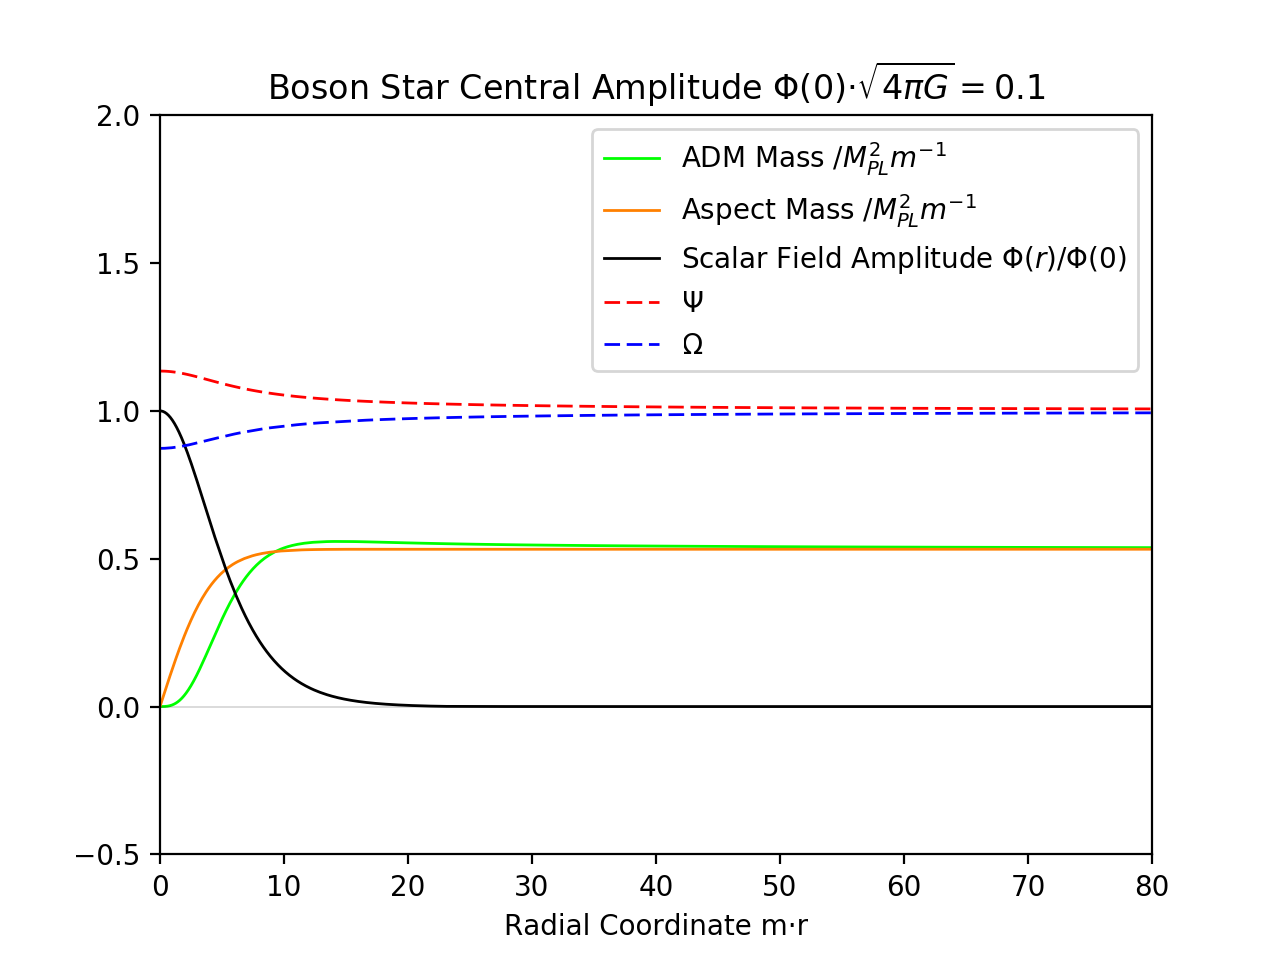
\includegraphics[width=0.5\textwidth]{bosonstar_groundstate.png}\label{boson:fig:f1}}
  \hfill
  \subfloat{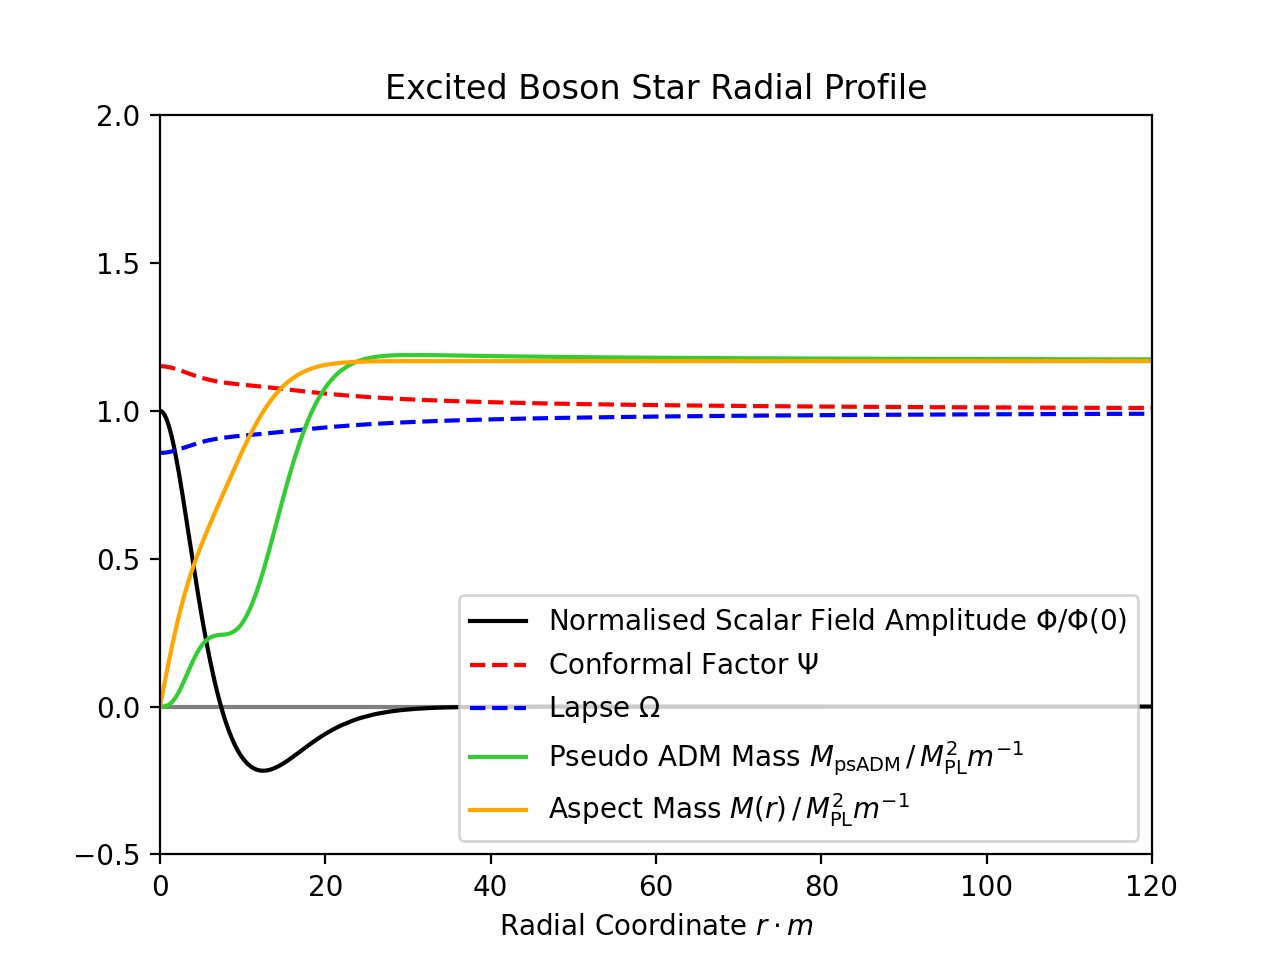
\includegraphics[width=0.5\textwidth]{bosonstar_excitedstate.png}\label{boson:fig:f2}}
\end{figure}

Figures () show the numerical result for the radial profile of a mini boson star ($\Lambda=0$) and an excited mini boson star. Note two mass definitions are plotted; the ADM mass (calculated as a function of finite r) and the aspect mass $M_A(r)$ which corresponds to assuming the metric's solution is Schwarzschild with $M_A(r)$ rather than $M$. Polytropic fluid stars were also simulated as a preliminary test of the code; they are much easier to create not needing to solve an eigenvalue problem and don't have an asymptotically growing mode. Figures () show how the ADM mass of boson stars varies with central amplitude $\Phi(0)$ and $r_{99}$, the radius which $\Phi(r_{99}) = \Phi(0)/100$. It should be noted that the $\Lambda =0$ case agrees with the known maximum mass, the Kaup limit [] $M_{max} \approx 0.633 {M_{PL}^2}{m^{-1}}$ with the highest measured mass being $ M_{max} = 0.63299(3) {M_{PL}^2}{m^{-1}} $ corresponding to a central amplitude of $\ \sqrt{4\pi G}\Phi(0)_{max} = 0.271(0)$. 

  \begin{figure}[H]
  \caption{Boson star trends, Left: ADM mass vs $\Phi(0)$, Right: ADM mass vs $r_{99}$}
  \centering
  \subfloat{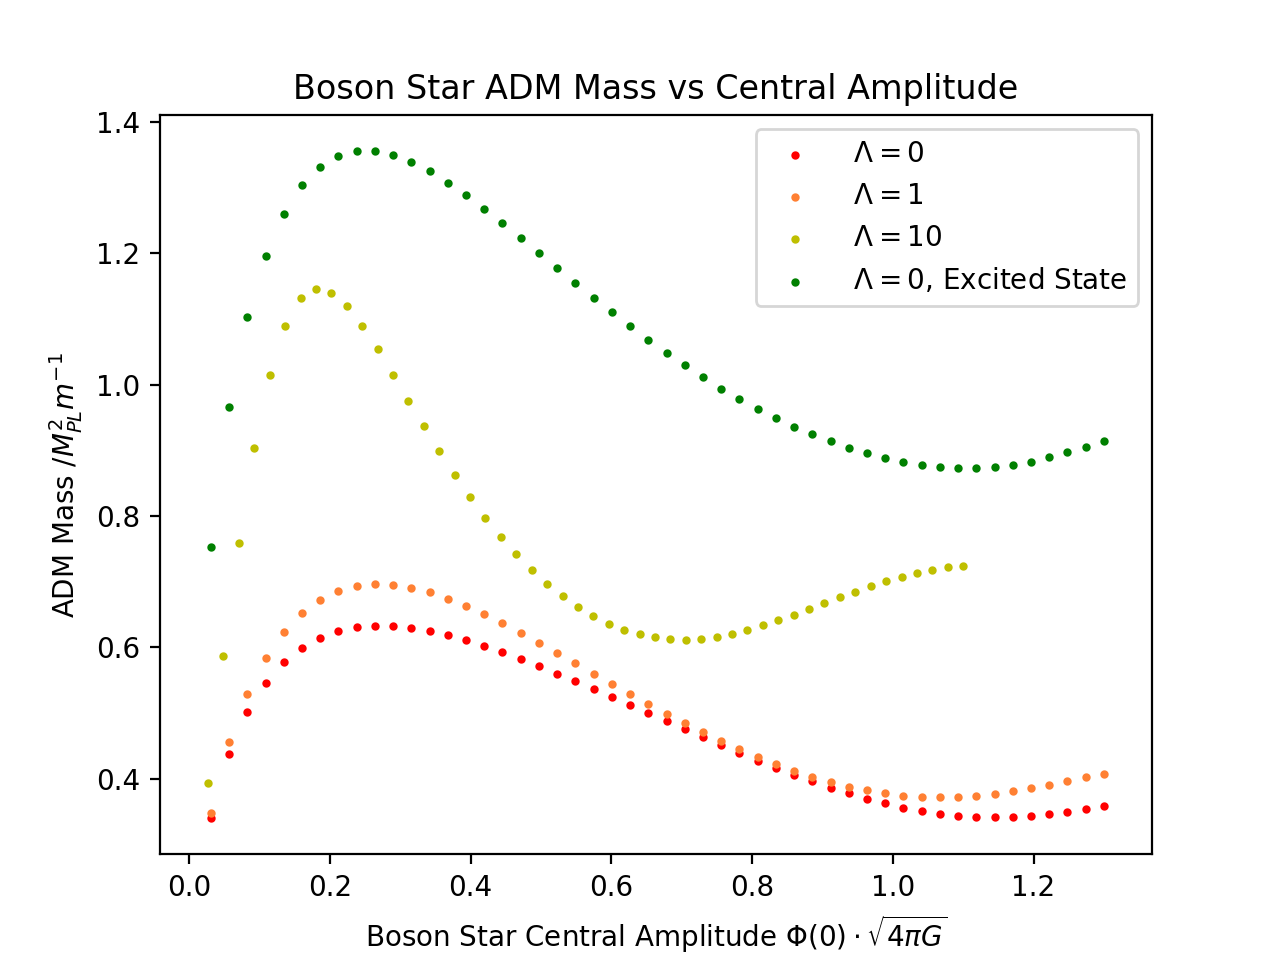
\includegraphics[width=0.5\textwidth]{ADM_vs_PC.png}\label{boson:fig:f1}}
  \hfill
  \subfloat{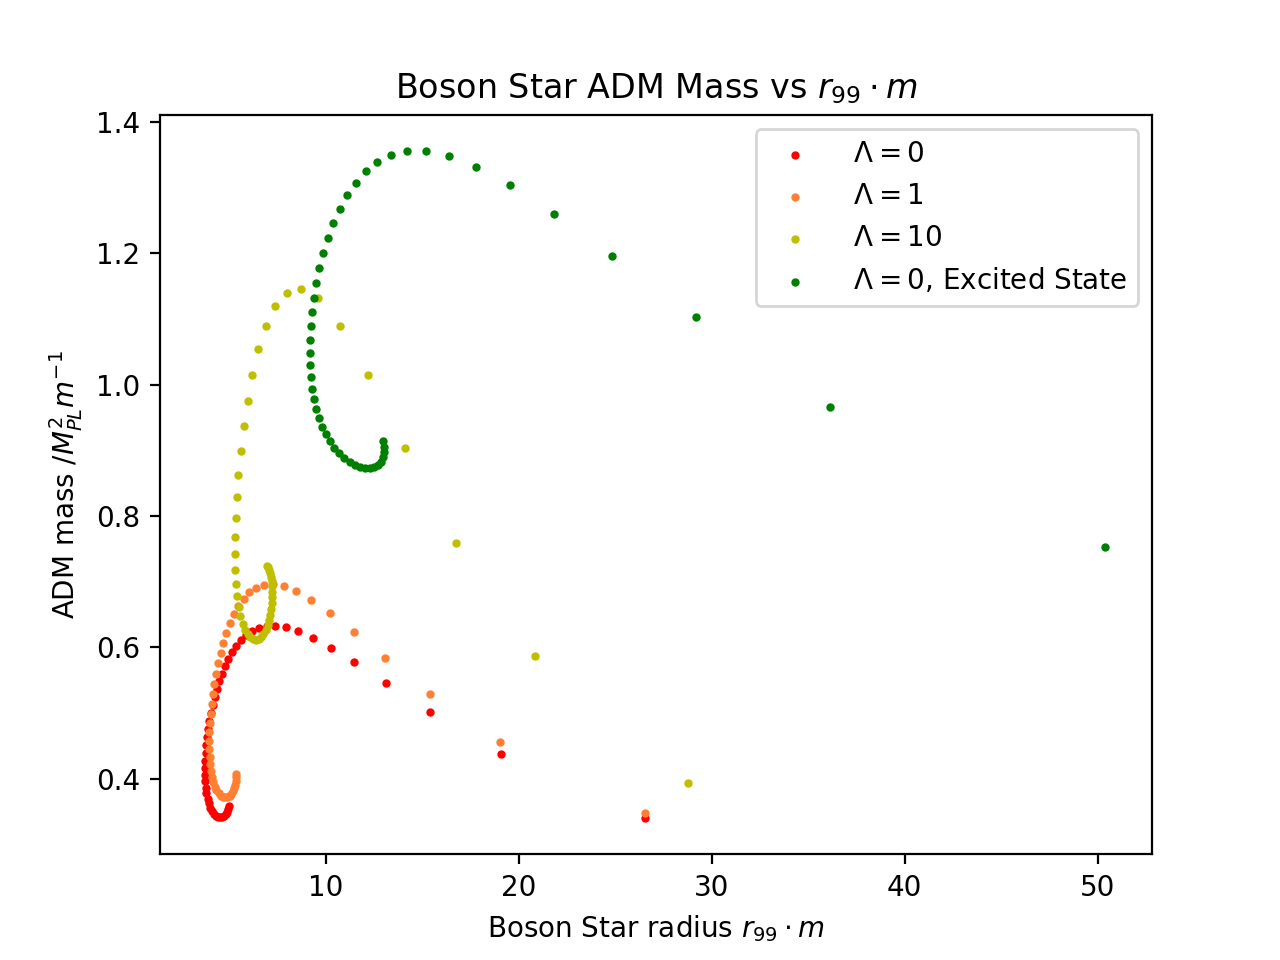
\includegraphics[width=0.5\textwidth]{ADM_vs_r99.png}\label{boson:fig:f2}}
\end{figure}

While many different boson stars have been made to test the initial data code, all the following evolutions use the same boson star with parameters $\Lambda=0$, $\sqrt{4\pi G}\Phi(0)=0.1 \rightarrow \Phi(0) \approx 0.0282$ and ADM mass $M=0.532(7)$. This is as the stars are heavy enough to form black holes under collisions and large deformations, but stable enough to not collapse to a black hole for moderate perturbations.


\subsection{Single Star Evolutions}
  \begin{figure}[H]
  \caption{Left: 2D slice of initial $|\vp|$, Right: Maximum of $|\vp|$ during evolution.}
  \centering
  \subfloat{\includegraphics[width=0.5\textwidth]{mod_phi_nice0000.png}\label{boson:fig:f1}}
  \hfill
  \subfloat{\includegraphics[width=0.5\textwidth]{modphimax.png}\label{boson:fig:f2}}
\end{figure}
The first simulation done was of the $\Phi(0)=0.02820$ mini boson star; as mentioned before all simulations are done with this star. The star is supposed to remain in the centre of the grid and not change as it is a rest frame soliton; this is observed through evolution with GRChombo. Figure () shows a rough initial phase in $|\vp|$ which changes significantly upon changing the AMR regridding, hence it is likely only a side effect of the interpolation errors at the boundary of AMR regions. Figure () shows that the star conserves $\mathcal{N}$ upto 4 figures and the constraint $\mathcal{H}$ is driven towards zero as desired.

  \begin{figure}[H]
  \caption{Left: Total Noether charge $\mathcal{N}$ during evolution, Right: $|| \mathcal{H} ||_2$ during evolution.}
  \centering
  \subfloat{\includegraphics[width=0.5\textwidth]{N.png}\label{boson:fig:f1}}
  \hfill
  \subfloat{\includegraphics[width=0.5\textwidth]{H.png}\label{boson:fig:f2}}
\end{figure}

\subsection{Superposition of Initial Data}
Suppose we have two compact objects with fields $\vp$, $\Pi$, $\gamma_{ij}$, $\K_{ij}$, $\alpha$ and $\beta^i$. The chosen scheme to superpose solutions is below.
\begin{gather*} \vp = \vp^{(1)} + \vp^{(2)}\\
\Pi = \Pi^{(1)} + \Pi^{(2)}\\
 \K^i_j = {\K^{(1)}}^i_j+{\K^{(2)}}^i_j\\
 \gamma_{\mu\nu} = \gamma^{(1)}_{\mu\nu} + \gamma^{(2)}_{\mu\nu}\\
\beta_i = \beta^{(1)}_i + \beta^{(2)}_i \\
 \alpha = \sqrt{\alpha_{(1)}^2 + \alpha_{(2)}^2-1} \quad \mathrm{or}\quad \left[ \alpha_{(1)}^{-1} +  \alpha_{(2)}^{-1}-1\right]^{-1}\\
 \chi = \det{\gamma^{(1)}_{\mu\nu} + \gamma^{(2)}_{\mu\nu}}^{-1/3}\end{gather*}
When a black hole is involved $\Omega(r=\frac{2}{M})=0$ so the event horizon causes the lapse to cross through zero; this is circumvented by setting
\begin{equation} \alpha = \sqrt{\chi}\end{equation}
and the lapse is real, non-negative for a spacelike hypersurface $\Sigma$. Superposing the scalar field $\vp$ is exact for the mini boson star (); for every other variable and type of star case superposition is inexact. Luckily, for sufficiently separated compact objects, superposition gives a very close approximation to the exact numerical solution. The use of CCZ4 also forces the evolution towards a constraint satisfying one. 



\subsection{Head-on Collisions}
All the cases studied here are for stationary initial data $\tilde{\A}_{ij}=0,\K=0$ in-falling from an initial separation of $d \cdot m = 32$ due to gravitational attraction. Firstly we consider the equal mass Boson star binary, initial data in figure (). At first they slowly infall creating a short lived object with three maxima, shown in figure (,left), then collapse to a black hole with a decaying spherical harmonic cloud (figures ) outside. As with all the simulations from now on we assume a black hole forms if $\chi \ll 16^{-1}$ where $\chi=16^-1$ is the value taken on the horizon for the isotropic Schwarzschild metric.
  \begin{figure}[H]
  \caption{Initial Data, Left: $\chi$, Right: $|\vp|$.}
  \centering
  \subfloat{\includegraphics[width=0.5\textwidth]{headon_bs/chi0000.png}\label{boson:fig:f1}}
  \hfill
  \subfloat{\includegraphics[width=0.5\textwidth]{headon_bs/modphi0000.png}\label{boson:fig:f2}}
\end{figure}
  \begin{figure}[H]
  \caption{Scalar field amplitude before and after black hole formation, Left: Time $t\cdot m = 150$, Right: Time $t \cdot m = 200$.}
  \centering
  \subfloat{\includegraphics[width=0.5\textwidth]{headon_bs/modphi0003.png}\label{boson:fig:f1}}
  \hfill
  \subfloat{\includegraphics[width=0.5\textwidth]{headon_bs/modphi0004.png}\label{boson:fig:f2}}
\end{figure}
   \begin{figure}[H]
  \caption{Real part of scalar field after black hole formation, Left: xy plane, Right: yz plane, perpendicular to initial star separation.}
  \centering
  \subfloat{\includegraphics[width=0.5\textwidth]{headon_bs/phi_re0004.png}\label{boson:fig:f1}}
  \hfill
  \subfloat{\includegraphics[width=0.5\textwidth]{headon_bs/phi_re_perp0004.png}\label{boson:fig:f2}}
\end{figure}
 
The second case considered is the same Boson star outside a black hole parameterised by $M=10M_{BS}$ where $M_{BS}$ is the ADM mass of the Boson star. The scalar field tidally deforms into an ellipsoid with high central density, well beyond Kaup limit of $\vp(0)\sim 0.0764$, and spontaneous collapse to a smaller external black hole is observed. After collapse, figure (), there is an elongated cloud about the new small black hole; there are many nodal lines in $\mathrm{Re}(\vp)$ which focus on the large black hole showing the cloud is in-falling.

  \begin{figure}[H]
  \caption{Initial Data, Left: $\chi$, Right: $|\vp|$.}
  \centering
  \subfloat{\includegraphics[width=0.5\textwidth]{LMR/chi0000.png}\label{boson:fig:f1}}
  \hfill
  \subfloat{\includegraphics[width=0.5\textwidth]{LMR/modphi0000.png}\label{boson:fig:f2}}
\end{figure}
  \begin{figure}[H]
  \caption{Final Data at time $t\cdot m = 125$, Left: Conformal factor $\chi$, Right: Scalar field modulus $|\vp|$, Bottom: Real part of scalarfield $\mathrm{Re}(\vp).$}
  \centering
  \subfloat{\includegraphics[width=0.5\textwidth]{LMR/chi0005.png}\label{boson:fig:f1}}
  \hfill
  \subfloat{\includegraphics[width=0.5\textwidth]{LMR/modphi0005.png}\label{boson:fig:f2}}
  \\
   \subfloat{\includegraphics[width=0.5\textwidth]{LMR/phi_re0000.png}\label{boson:fig:f2}}
\end{figure}
Final case consists of an equal mass Black Hole and Boson Star, initial configuration in Figure 11. As can be seen from the plot of $\Re(\phi)$ and $|\phi|$, in Figure 12, most of the star falls into the black hole, however some scalar field manages to excite an intricate spherical harmonic cloud pattern.
  \begin{figure}[H]
  \caption{Initial data for equal mass Boson Star and Black Hole, Left: $\chi$, Right: $|\vp|$}
  \centering
  \subfloat{\includegraphics[width=0.5\textwidth]{headon/chi0000.png}\label{boson:fig:f1}}
  \hfill
  \subfloat{\includegraphics[width=0.5\textwidth]{headon/mod_phi0000.png}\label{boson:fig:f2}}
\end{figure}
  \begin{figure}[H]
  \caption{Time $t\cdot m=905$ for equal mass Boson Star and Black Hole, Left: $\Re(\vp)$, Right: $|\vp|$}
  \centering
  \subfloat{\includegraphics[width=0.5\textwidth]{headon/phi_re0000.png}\label{boson:fig:f1}}
  \hfill
  \subfloat{\includegraphics[width=0.5\textwidth]{headon/mod_phi0007.png}\label{boson:fig:f2}}
\end{figure}

In all three cases, the Noether charge drops rapidly upon the formation of a black hole; this will be explained in the next section. However some scalar field lingers after collapse, in each case the hair takes the form of spherical harmonics discussed in (). Also observed is the decay of the spherical harmonics to zero amplitude in these simulations with no angular momentum. 
 
\subsection{Binary Inspiral}
The only considered case here is the Quasi-circular orbit and inspiral of two equal mass boson stars. The initial boosts were determined by a newtonian calculation yielding 
\begin{equation} v^2 = \frac{M}{2d}\end{equation}
where $M=0.53(29)$ is the ADM mass of the Boson Star and d is the initial separation. For a relatively low separation of $d\cdot m =32$ code units, shown in Figures 13,14 (Left), we get $v \sim 0.0915$. The boson stars are observed to complete roughly half an orbit before merging and collapse, forming a black hole. Here a Kerr black hole is assumed to have formed as the spacetime has a significant angular momentum which should partially infall with the scalar field. 

  \begin{figure}[H]
  \caption{Boson Star $|\vp|$. Left: initial data, Right: later time $t \cdot m = 700$}
  \centering
  \subfloat{\includegraphics[width=0.5\textwidth]{inspiral/mod_phi_inspiral_nice0000.png}\label{boson:fig:f1}}
  \hfill
  \subfloat{\includegraphics[width=0.5\textwidth]{inspiral/mod_phi_inspiral_nice0002.png}\label{boson:fig:f2}}
\end{figure}
  \begin{figure}[H]
  \caption{Boson Star $\Re(\vp)$. Left: initial data, Right: later time $t \cdot m = 700$}
  \centering
  \subfloat{\includegraphics[width=0.5\textwidth]{inspiral/phi_inspiral_nice0000.png}\label{boson:fig:f1}}
  \hfill
  \subfloat{\includegraphics[width=0.5\textwidth]{inspiral/phi_inspiral_nice0002.png}\label{boson:fig:f2}}
\end{figure}
  \begin{figure}[H]
  \caption{Left: Total Noether charge $\mathcal{N}$ during evolution, Right: $\Psi_4$ over 22 harmonic during evolution.}
  \centering
  \subfloat{\includegraphics[width=0.5\textwidth]{inspiral/N.png}\label{boson:fig:f1}}
  \hfill
  \subfloat{\includegraphics[width=0.5\textwidth]{inspiral/GW.png}\label{boson:fig:f2}}
\end{figure}
Figure 15 shows the total Noether charge, which is no longer conserved. When the black hole forms, the in-falling scalar field moves towards zero radius and gets hugely compressed. The huge compression causes extreme field gradients which induces continuous regridding in the AMR, but this is capped at 7 layers in this simulation to make runtime feasible. When the 8th AMR level is needed it is simply not added and resolution becomes low enough that any Noether charge near the centre is so under-resolved that it seems to fall between the gridpoints. Interestingly, Figures 13,14 (Right) show a scalar field configuration lingering around the black hole, mostly outside the contour $\chi=0.7$, looking like scalar hair. Also Figure 15 (Left) of the Noether charge appears to take significantly longer to decay than in the linear collision simulations. It can be seen in Figure 14 in the plot of $\Re(\vp)$ that the cloud has angular nodes corresponding to angular momentum similarly to boosted stars picking up nodal planes perpendicular to momentum and Figure 10 (Bottom) of the infalling cloud. 

The gravitational wave (GW) signal can be seen in Figure 15 (Right), extracted at a radius $r \cdot m = 90$. At the time $t \cdot m \approx 700$ the gravitational wave signal due to the merger appears; in order to record a longer inspiral simulations with larger initial separations need to be simulated. Currently there appears to be some small problem with the initial data, also observed in the collisions with no angular momentum, that manifests itself in noisy GW extraction and the Hamiltonian constraint initially sharply rising. 



\subsection{stuff}
FIX THE FUCKING HAND REFERNECES!

\end{document}